\documentclass[aspectratio=169]{beamer}
\usepackage[utf8]{inputenc}
\usefonttheme{serif}
\usetheme{boxes}
\setbeamertemplate{frametitle}[default][center]
\setbeamersize{text margin right=20mm, text margin left=20mm} 
\addtobeamertemplate{frametitle}{\vskip1cm}{}
\setbeamertemplate{navigation symbols}{}

%% absolute positioning
\usepackage[absolute,overlay]{textpos}
\usepackage{mathrsfs} % https://www.ctan.org/pkg/mathrsfs

\usepackage{xspace}
\usepackage[version=0.96]{pgf}
\usepackage{tikz}
\usetikzlibrary{fit,shapes.geometric,calc,decorations.pathmorphing}
%Information to be included in the title page:
\title{\bf\LARGE Papers We Love \color{gray}{Milano} \#4}
\subtitle{Partial Computation of Programs\\[5pt] (Futamura 1984)}
\author{Edoardo Vacchi}
% \institute{Overleaf}
\date{19th February 2020}

\renewcommand{\P}{\ensuremath{\mathcal{P}}\xspace}
\newcommand{\C}{\ensuremath{\mathcal{C}}\xspace}
\newcommand{\I}{\ensuremath{\mathcal{I}}\xspace}
\newcommand{\D}{\ensuremath{\mathcal{D}}\xspace}
\newcommand{\R}{\ensuremath{\mathcal{R}}\xspace}
 
\begin{document}
 
\frame{\titlepage}



\begin{frame}{Programs}

    \begin{itemize}
        \item Consider a program \P, with input data \D;
        \item when we \textit{evaluate} \P over \D it produces
        some output result \R.
    \end{itemize}



    \begin{center}
    
        \begin{tikzpicture}
            \tikzstyle{every path}=[draw, ->]
            \tikzstyle{circ}=[draw, circle]
            \tikzstyle{box}=[draw, rectangle, text width=1cm, text height=.5cm, text centered, text depth=.3cm]
                \node [circ] (d) at (2,2) {\D};    
                \node [circ] (r) at (8,2) {\R};    
                \node [box] (p) at (5,2) {\footnotesize$ eval(\P)$}; 
                \path (d) -- (p);    
                \path (p) -- (r);    
        \end{tikzpicture}
        
    \end{center}

    
\end{frame}

\begin{frame}{Interpreters}

    \begin{itemize}
    \item An \textit{interpreter} $\mathcal{I}$ is a \textit{program} 
    \item it \textit{evaluates} some other given program $\mathcal{P}$
    over some given data $\mathcal{D}$, and it produces the output
    result \R.
    \end{itemize}


\begin{center}

    \begin{tikzpicture}
        \tikzstyle{every path}=[draw, ->]
        \tikzstyle{circ}=[draw, circle]
        \tikzstyle{box}=[draw, rectangle, text width=1cm, text height=.5cm, text centered, text depth=.3cm]
            \node [circ] (p) at (2,3) {\P};    
            \node [circ] (d) at (2,1) {\D};    
            \node [circ] (r) at (8,2) {\R};    
            \node [box] (i) at (5,2) {\I}; 
            \path (p) -- (i);    
            \path (d) -- (i);    
            \path (i) -- (r);    
    \end{tikzpicture}
    
\end{center}


\end{frame}



\begin{frame}{Compilers}

    \begin{itemize}

        \item 
            Let be \P a program that evaluates to \R when given \D;
        \item  
            A \textit{compiler}, say $\mathcal{C}$, translates a source program
            $\mathcal{P}$ to an object program $\P'$ that
            evaluated over an input \D still produces \R
        
    
    
    \end{itemize}




    \begin{center}
    
        \begin{tikzpicture}
            \tikzstyle{every path}=[draw, ->]
            \tikzstyle{circ}=[draw, circle]
            \tikzstyle{box}=[draw, rectangle, text width=1cm, text height=.5cm, text centered, text depth=.3cm]
                \node [circ] (p)   at (2,2) {\P};    
                \node [box]  (c)   at (5,2) {\C}; 
                \node [circ] (cp)  at (8,2) {$\P'$};    
                \node [box]  (cp2) at (5,0) {$\P'$};    
                \node [circ] (d)   at (2,0) {\D};    
                \node [circ] (r)   at (8,0) {\R};    
                \path (p) -- (c);    
                \path (c) -- (cp);    
                \path (d) -- (cp2);    
                \path (cp2) -- (r);    
        \end{tikzpicture}
        
    \end{center}

\end{frame}

\begin{frame}
    
    Now, if we indicate $\P'$ with $C(P)$ we can write the following:

    \begin{eqnarray*}        
        \P(\D) &=& \R\\
        \C(\P) &=& \P'\\
        \P'(\D) &=& \R\\
        \C(\P)(\D) &=& \R\\
        \I(\P, \D) &=& \R\\
        \C(\P)(\D) &=& \I(\P, \D) \\
    \end{eqnarray*}
    
\end{frame}

% \begin{frame}{Compilers and Interpreters}

%     \begin{itemize}
%         \item 
%             An \textit{interpreter} $\mathcal{I}$ is a program to perform
%             specified computations that analyze the meanings of a given program, 
%             say $\mathcal{P}$, based upon given data, say $\mathcal{D}$.

%         \item 
%             A \textit{compiler}, say $\mathcal{C}$, translates a source program
%             say $\mathcal{P}$, to an object program $\mathcal{C}(\mathcal{P})$
        
    
    
%     \end{itemize}
    
%     Thus, 
%     running a program by intepreter means performing $\mathcal{I}(\mathcal{P}, \mathcal{D})$
    
    
%     This produces the following equation:
    
%     \[
%         \mathcal{C}(\mathcal{P})(\mathcal{D}) = \mathcal{I}(\mathcal{P},\mathcal{D})
%     \]
    
%     while $ \mathcal{I}_{\mathcal{P}} =  \alpha(\mathcal{I},\mathcal{P}) $
    
%     \begin{equation}
%     \mathcal{I}_{\mathcal{P}} =  \mathcal{C}(\mathcal{P})
%     \end{equation}
    
    
% \end{frame}

\begin{frame}{Partial Evaluation (intuition)}
    Let us have a computation $f$ of two parameters $k$, $u$
    \[
        f(k,u)
    \]
    \begin{itemize}
    \item Now suppose that $f$ is often called with $k=5$; 
    
    \item we may define the program $f_5(u)$ by substituting $5$ for $k$ in $f$ 
    and doing all possible computation based upon value $5$.

    \item  Partial evaluation is the process of rewriting $f(5,u)$ into $f_5(u)$
    \end{itemize}
\end{frame}
 


\begin{frame}

    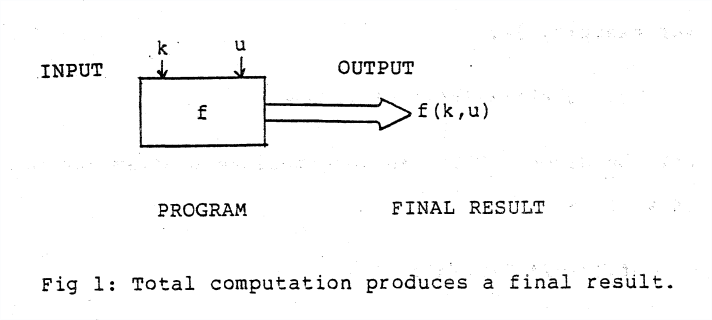
\includegraphics[width=\textwidth]{imgs/fig1.png}

\end{frame}
 


\begin{frame}

    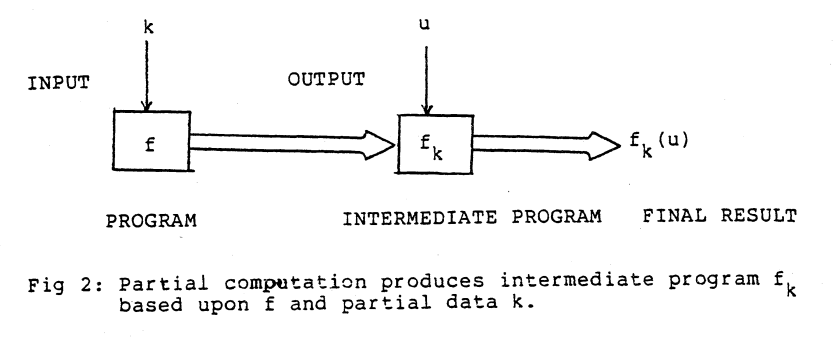
\includegraphics[width=\textwidth]{imgs/fig2.png}

\end{frame}
 
\begin{frame}{Projection}
Consider $f$

    \[
        f(k,u) \triangleq k \cdot ( k \cdot (k+1) + u + 1) + u\cdot u
    \]

now let $k=2$, we can write $f_2$ as follows

    \[
        f_2(u) \triangleq 2 \cdot (7+u) + u\cdot u    
    \]

because $f(2,u) = f_2(u)$ for any value of $u$, 
the following equation holds for $f_k$ and $f$



    \begin{equation}
        f_k(u)=f(k,u)
    \end{equation}

And we call it \textit{a projection of $f$ at $k$}

\end{frame}

\begin{frame}{Partial Evaluator}

A partial computation procedure may be a computer program $\alpha$
called \textit{a projection machine}, \textit{partial computer} 
or \textit{partial evaluator}.

\begin{equation}
    \alpha(f,k) = f_k
\end{equation}

\end{frame}

\begin{frame}{Partial Evaluator (diagram)}
    
\begin{center}

    \begin{tikzpicture}
        \tikzstyle{every path}=[draw, ->]
        \tikzstyle{envel}=[shape=ellipse, draw]
        \tikzstyle{circ}=[draw, circle]
        \tikzstyle{box}=[draw, rectangle, text width=1cm, text height=.5cm, text centered, text depth=.3cm]
            \node [circ] (in1) at (2,3) {$k$};    
            \node [circ] (in2) at (2,1) {$f$};    
            \node [circ] (out) at (8,2) {$f(k,u)$};    
            \node [box] (box) at (5,2) {$f$};
            
            
            \path (in1) -- (box);    
            \path (in2) -- (box);    
            \path (box) -- (out);

            \pause

            \begin{scope}[shift={(in1))},x={(box)},y={($(in1)!1!90:(box)$)}]
                \draw[red] (.5,0) ellipse (.8 and .5);
            \end{scope}

            \pause

            \node[box](proj) at (5,-.5) {$f_k$};

            \draw[
                line join=round,
                decorate, decoration={
                zigzag,
                segment length=4,
                amplitude=1,post=lineto,
                post length=2pt}] (5,.9) -- (proj) node [midway, label=right:{$\alpha$}] {} ;
            
    \end{tikzpicture}
    
\end{center}


\end{frame}


\begin{frame}{Basic Equation of Partial Evaluation}

Non consider $\alpha_f$, the partial evaluation of $\alpha$ at $f$; then:

\begin{eqnarray*}
            &\alpha_f(k) &= \alpha(f,k)\\
            &\alpha(f,k) &= f_k
\end{eqnarray*}

therefore:
\begin{equation}
       \alpha_f(k) =f_k 
\end{equation}
\end{frame}

\begin{frame}{Automatically generating a compiler}

    \begin{itemize}
        \item Automatic theorem proving
        \item Pattern matching
        \item Syntax analyzer
        \item Automatically generating a compiler
    \end{itemize}
    
\end{frame}




\begin{frame}{Partial Evaluation of an Interpreter}


\begin{center}

    \begin{tikzpicture}
        \tikzstyle{every path}=[draw, ->]
        \tikzstyle{envel}=[shape=ellipse, draw]
        \tikzstyle{circ}=[draw, circle]
        \tikzstyle{box}=[draw, rectangle, text width=1cm, text height=.5cm, text centered, text depth=.3cm]
            \node [circ] (in1) at (2,3) {\P};    
            \node [circ] (in2) at (2,1) {\D};    
            \node [circ] (out) at (8,2) {\R};    
            \node [box] (box) at (5,2) {\I};
            
            
            \path (in1) -- (box);    
            \path (in2) -- (box);    
            \path (box) -- (out);

            \pause

            \begin{scope}[shift={(in1))},x={(box)},y={($(in1)!1!90:(box)$)}]
                \draw[red] (.5,0) ellipse (.8 and .5);
            \end{scope}

            \pause

            \node[box](proj) at (5,-.5) {$\I_\P$};

            \draw[
                line join=round,
                decorate, decoration={
                zigzag,
                segment length=4,
                amplitude=1,post=lineto,
                post length=2pt}] (5,.9) -- (proj) node [midway, label=right:{$\alpha$}] {} ;
            
    \end{tikzpicture}
    
\end{center}

\end{frame}


\begin{frame}{Partially Evaluated Interpreter}
    \begin{center}
    
        \begin{tikzpicture}
            \tikzstyle{every path}=[draw, ->]
            \tikzstyle{circ}=[draw, circle]
            \tikzstyle{box}=[draw, rectangle, text width=1cm, text height=.5cm, text centered, text depth=.3cm]
                \node [circ] (in) at (2,2) {\D};    
                \node [circ] (out) at (8,2) {\R};    
                \node [box] (box) at (5,2) {$\I_\P$}; 
                \path (in) -- (box);    
                \path (box) -- (out);    
        \end{tikzpicture}
        
    \end{center}

    \begin{itemize}
    \item That is, by feeding \D into $\I_\P$, you get \R;
    \item in other words, $\I_\P$ is \textit{an object program}.
    \end{itemize}
    
\end{frame}


\begin{frame}{First Equation of Partial Computation (First Projection)}

    
% An \textit{interpreter} $\mathcal{I}$ is a program to perform
% specified computations that analyze the meanings of a given program, 
% say $\mathcal{P}$, based upon given data, say $\mathcal{D}$. 

We recall the previous definitions of \textit{interpreter}
and \textit{compiler}.

\begin{eqnarray}
    \mathcal{I}(\mathcal{P}, \mathcal{D}) &=& \R \nonumber \\
    \C(\P)&=&\P' \nonumber \\
    \P' &=& \R \nonumber  \\
    \mathcal{C}(\mathcal{P})(\mathcal{D}) &=& \mathcal{I}(\mathcal{P},\mathcal{D}) \nonumber \\
    \mathcal{I}_{\mathcal{P}} &=&  \alpha(\mathcal{I},\mathcal{P}) \nonumber \\ 
    \mathcal{I}_{\mathcal{P}} &=&  \mathcal{C}(\mathcal{P})
\end{eqnarray}


\end{frame}

\begin{frame}{Partial Evaluation of an Interpreter}

    \begin{center}
    
        \begin{tikzpicture}
            \tikzstyle{every path}=[draw, ->]
            \tikzstyle{envel}=[shape=ellipse, draw]
            \tikzstyle{circ}=[draw, circle]
            \tikzstyle{box}=[draw, rectangle, text width=1cm, text height=.5cm, text centered, text depth=.3cm]
                \node [circ] (in1) at (2,3) {\I};    
                \node [circ] (in2) at (2,1) {\P};    
                \node [circ] (out) at (8,2) {$\I_\P$};    
                \node [box] (box) at (5,2) {$\alpha$};
                
                
                \path (in1) -- (box);    
                \path (in2) -- (box);    
                \path (box) -- (out);
    
                \pause
    
                \begin{scope}[shift={(in1))},x={(box)},y={($(in1)!1!90:(box)$)}]
                    \draw[red] (.5,0) ellipse (.8 and .5);
                \end{scope}
    
                \pause
    
                \node[box](proj) at (5,-.5) {$\alpha_\I$};
    
                \draw[
                    line join=round,
                    decorate, decoration={
                    zigzag,
                    segment length=4,
                    amplitude=1,post=lineto,
                    post length=2pt}] (5,.9) -- (proj) node [midway, label=right:{$\alpha$}] {} ;
                
        \end{tikzpicture}
        
    \end{center}
    
    \end{frame}


\begin{frame}{Second Equation of Partial Computation (Second Projection)}

    

    \begin{center}
    
        \begin{tikzpicture}
            \tikzstyle{every path}=[draw, ->]
            \tikzstyle{circ}=[draw, circle]
            \tikzstyle{box}=[draw, rectangle, text width=1cm, text height=.5cm, text centered, text depth=.3cm]
                \node [circ] (in) at (2,2) {\P};    
                \node [circ] (out) at (8,2) {$\I_\P$};    
                \node [box] (box) at (5,2) {$\alpha_\I$}; 
                \path (in) -- (box);    
                \path (box) -- (out);    
        \end{tikzpicture}
        
    \end{center}


    \begin{equation}
    \alpha_\mathcal{I}(\mathcal{P}) =  \mathcal{I}_\mathcal{P}
    \end{equation}
    
    \begin{itemize}
        \item but $\I_\P$, evaluated on \D gives \R; then
        \item $\I_\P$ is an object program ($\P'$)
        \item $\alpha_\I$ transforms a source program $\P$ to $\I_\P$
        \item then $\alpha_\I$ is \textit{a compiler}
    \end{itemize}
    
\end{frame}



\begin{frame}{Partial Evaluation of a Partial Evaluator}


    \begin{center}
    
        \begin{tikzpicture}
            \tikzstyle{every path}=[draw, ->]
            \tikzstyle{envel}=[shape=ellipse, draw]
            \tikzstyle{circ}=[draw, circle]
            \tikzstyle{box}=[draw, rectangle, text width=1cm, text height=.5cm, text centered, text depth=.3cm]
                \node [circ] (in1) at (2,3) {$\alpha$};    
                \node [circ] (in2) at (2,1) {\I};    
                \node [circ] (out) at (8,2) {$\alpha_\I$};    
                \node [box] (box) at (5,2) {$\alpha$};
                
                
                \path (in1) -- (box);    
                \path (in2) -- (box);    
                \path (box) -- (out);
    
                \pause
    
                \begin{scope}[shift={(in1))},x={(box)},y={($(in1)!1!90:(box)$)}]
                    \draw[red] (.5,0) ellipse (.8 and .5);
                \end{scope}
    
                \pause
    
                \node[box](proj) at (5,-.5) {$\alpha_\alpha$};
    
                \draw[
                    line join=round,
                    decorate, decoration={
                    zigzag,
                    segment length=4,
                    amplitude=1,post=lineto,
                    post length=2pt}] (5,.9) -- (proj) node [midway, label=right:{$\alpha$}] {} ;
                
        \end{tikzpicture}
        
    \end{center}
    
    \end{frame}


\begin{frame}{Third Equation of Partial Computation (Third Projection)}

    \begin{center}
    
        \begin{tikzpicture}
            \tikzstyle{every path}=[draw, ->]
            \tikzstyle{circ}=[draw, circle]
            \tikzstyle{box}=[draw, rectangle, text width=1cm, text height=.5cm, text centered, text depth=.3cm]
                \node [circ] (in) at (2,2) {\I};    
                \node [circ] (out) at (8,2) {$\alpha_\I$};    
                \node [box] (box) at (5,2) {$\alpha_\alpha$}; 
                \path (in) -- (box);    
                \path (box) -- (out);    
        \end{tikzpicture}
        
    \end{center}

    \begin{equation}
    \alpha_\alpha(\mathcal{I}) =  \alpha_\mathcal{I}
    \end{equation}
    
    \begin{itemize}
     \item $\alpha_\alpha$ is a program, that given \I, returns $\alpha_\I$
     \item $\alpha_\I$ transforms a source program to an object program
     \item $\alpha_\I$ is a compiler
     \item $\alpha_\alpha$ is a \textit{compiler-compiler} (a \textit{compiler generator})
            which generates a compiler $\alpha_\I$ from an interpreter $\I$
    \end{itemize}
\end{frame}

\begin{frame}{Partial Evaluation of a Partially-Evaluated Evaluator}

    \begin{itemize}
    \item Let us call \I-language a language implemented by interpreter \I,  
    \item let us now substitute $\alpha$ for $\I$ in $\alpha_\alpha(\mathcal{I}) = \alpha_\mathcal{I}$,
    \item which means considering $\alpha$ an interpreter for the $\alpha$-language.
    \end{itemize}

    \[
        \alpha_\alpha(\alpha)=\alpha_\alpha    
    \]


\end{frame}

\begin{frame}{Fourth Equation of Partial Computation}

    \[
        \alpha_\alpha(\alpha)=\alpha_\alpha    
    \]

    \begin{center}
    
        \begin{tikzpicture}
            \tikzstyle{every path}=[draw, ->]
            \tikzstyle{circ}=[draw, circle]
            \tikzstyle{box}=[draw, rectangle, text width=1cm, text height=.5cm, text centered, text depth=.3cm]
                \node [circ] (in) at (2,2) {$\alpha$};    
                \node [circ] (out) at (8,2) {$\alpha_\alpha$};    
                \node [box] (box) at (5,2) {$\alpha_\alpha$}; 
                \path (in) -- (box);    
                \path (box) -- (out);    
        \end{tikzpicture}
        
    \end{center}
    


    \begin{itemize}
    \item $\alpha_\alpha$ is an $\alpha$-language compiler.
    \item $\alpha_\alpha(f)$ is an object program of $f$; thus:
    \end{itemize}

    \begin{equation}
    \alpha_\alpha(f)(k) =  f_k
    \end{equation}
    
    
\end{frame}

\begin{frame}

    \begin{itemize}
    \item In other words, by finding $\alpha_\alpha$ we can generate
    the partial computation of $f$ at $k$, $f_k$
    
    \item That is, $\alpha_\alpha$ is a \textit{partial evaluation compiler}.

    \item However, \textit{the author notes}, at the time of writing, 
    there is no way to produce $\alpha_\alpha$ from $\alpha(\alpha, \alpha)$
    for practical $\alpha$'s.
    \end{itemize}

\end{frame}

\begin{frame}{Theory of Partial Computation}

\end{frame}

\begin{frame}
    \begin{enumerate}
        \item Correctness: 
            Program $\alpha$ must satisfy $\alpha(f,k)(u)=f(k,u)$
        \item Efficiency Improvement: 
            Program $\alpha$ should perform as much computation as possible
            for the given data $k$
        \item Termination:
            Program $\alpha$ should terminate on partial computation of as 
            many programs as possible. Termination at $\alpha(\alpha,\alpha)$ 
            is most desirable
    \end{enumerate}

However, author notes, (2) is not \textit{mathematically clear}

\end{frame}

\begin{frame}{Recursive Program Schema}
    \begin{enumerate}
        \item Condition
        \item Expression
        \item Function Definition
    \end{enumerate}


    \begin{enumerate}
        \item Rewriting
        \item Simplification
    \end{enumerate}

    Partial Computation

    \begin{enumerate}
        \item Rewriting
        \item Simplification
        \item Tabulation
    \end{enumerate}

    The discriminating character for p.c. are the semi-bound call and tabulation.

\end{frame}

\begin{frame}{Technical Problems in Making $\alpha$ Practical}

\end{frame}

     
\end{document}
    